%!TEX root = main.tex


In this section, we empirically evaluate the effectiveness and the efficiency of the
state-of-arts in deep reinforcement learing on OpenAI gym Atari environment. Note 
that at current stage, we didn't propose any new methods in deep reinforcement learning;
instead our first stage is to learning the most advanced algorithms first using public
available online resources. 


\subsection{Environments}

In order to evaluate the algorithm, we conduct our experiments on Atari environment
provided by OpenAI. The description of Atari environment is as follows:
\begin{quote}
Maximize your score in the Atari 2600 game. In this
environment, the observation is an RGB image of the screen, which is an array
of shape (210, 160, 3) Each action is repeatedly performed for a duration of
kk frames, where kk is uniformly sampled from \{2, 3, 4\}~\cite{brockman2016openai}
\end{quote}

We choose three Atari games as our testing environment, all of which are unsolved environments, 
which means those games don't have a specific reward that you can consider it as the end of game:

\begin{enumerate}
\item Breakout-v0\\
In this game, player control a paddles at the bottom of screen and try to bounce the ball upwards
to hit those bricks as soon and as much as possible, as illustrated in Fig~\ref{fig:A3C_baselines} (a). 

\item Pong-v0\\
In this game, players control a paddles at the right of screen and try to bounce the ball pass the
other player at the left of screen, as illustrated in Fig~\ref{fig:A3C_baselines} (b). 

\item Phoenix-v0
In this game, players control a spaceship by moving it horizontally at the bottom of screen, as 
illustrated in Fig~\ref{fig:A3C_baselines} (c), trying to destroy the enemies by firing upwards 
and avoiding the attack from those enemies. 
\end{enumerate}

\subsection{Baselines}

In this section, we introduce the implementation details of the baselines we used.

% As we introduced in Methodology section, we use two neural network to model policy function
% and value function, respectively. 
The structure of policy network is shown as in Table.\ref{table.cnn_detail}:

\begin{table}[!ht]
	\centering
	\caption{CNN detail}
	\label{table.cnn_detail}
	\begin{tabular}{c|c|c|c}
		\textbf{Type} & \textbf{size} & \textbf{\# filters} & \textbf{activation} \\ \hline
		convolution & $5\times5$ & 32 & Relu \\ 
		max pooling & $2\times2$ &  &  \\
		convolution & $5\times5$ & 32 & Relu \\
		max pooling & $2\times2$ &  &  \\
		convolution & $4\times4$ & 64 & Relu \\
		max pooling & $2\times2$ &  &  \\
		convolution & $3\times3$ & 64 & Relu \\
		fully connected & 512 &  & PRelu \\
		softmax &  &  & 
	\end{tabular}
\end{table}
%\begin{enumerate}
%\item Convolution layer: $(5 \times 5, 32)$ 
%\item Maximum pooling layer: $(2 \times 2) $
%\item Convolution layer: $(5 \times 5, 32)$ 
%\item Maximum pooling layer: $(2 \times 2) $
%\item Convolution layer: $(4 \times 4, 64)$ 
%\item Maximum pooling layer: $(2 \times 2) $
%\item Convolution layer: $(3 \times 3, 64)$ 
%\item Fully connected layer with 512 nodes and PReLU activation function.
%\item Softmax layer to predict the probability over all possible actions.
%\end{enumerate}
We modified the implementation of A3C from \href{https://github.com/ppwwyyxx/tensorpack}{tensorpack} repository.


\subsection{experimental results}




\subsubsection{Policy Gradient}
%!TEX root = main.tex

The results of policy gradient method on CartPole environment is show
in Figure~\ref{fig:pg_cartpole}. Also, a video illustration can be found
in \href{https://gym.openai.com/evaluations/eval_UaXIaMm1QxPGgW45KHtTA#reproducibility}{this link}.
As we can see in both the video and the figure, the game was solved by 
few hundred episodes. This show the effectiveness of policy gradient methods
and we further train a this model in a more complex environment. 

\begin{figure}[h!]
\centering
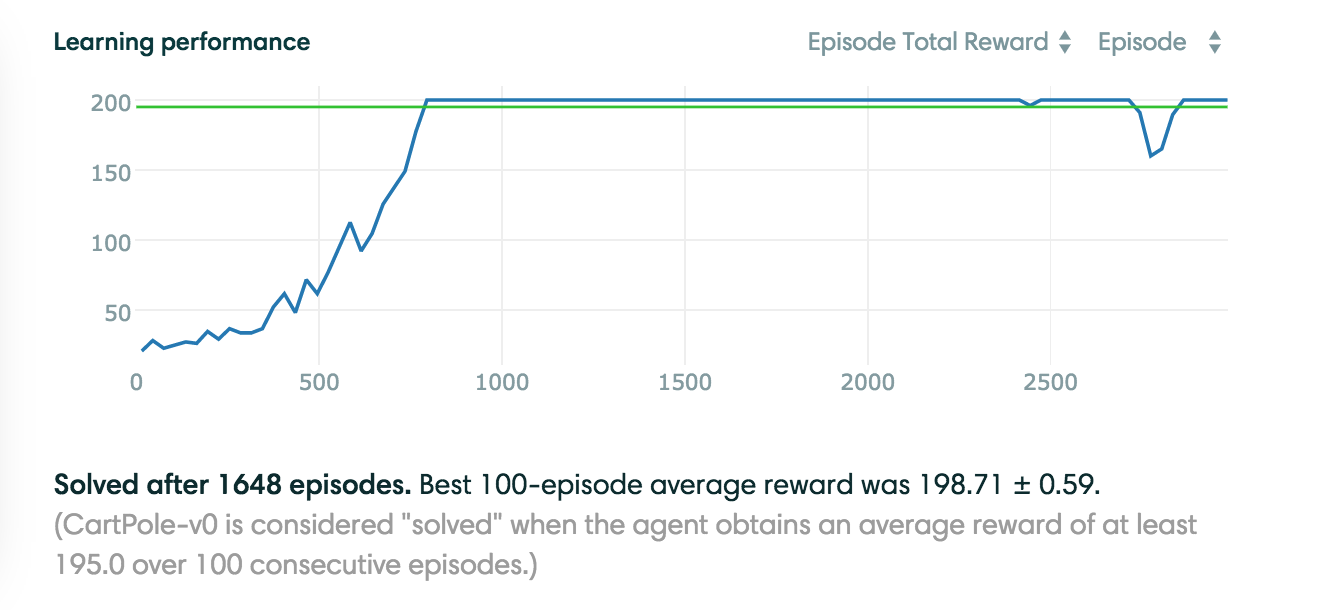
\includegraphics[width=0.49\textwidth]{./fig/pg_cartpole.png} 
\caption{The plot of reward for cartpole game. The x-axis is the number
of episodes it has been trained. The y-axis is the cumulative reward in 
per episode. The higher the better. }
\label{fig:pg_cartpole}
\end{figure}


The performance on Pong game is plot in Figure~\ref{fig:pg_pong} and a video
illustration can be found \href{https://gym.openai.com/evaluations/eval_dODFoXO2S4y5TuUZMX7Nw}{at this link}. As it
shown in the figure, this game requires more than 10000 episodes to get 
a model better than the baseline provided by OpenAI gym. It much more complicated
than the CartPole, since the state and action space is more complex than 
that. The structure of this policy is a single hidden layer with eight
hidden nodes fully connected network and it works. It may perform
better if we use a convolutional network to replace this one, but compared 
the results in dueling DQN, it seems the algorithms of reinforcement learning
itself is more important, other than the specific network architecture. 

\begin{figure}[h!]
\centering
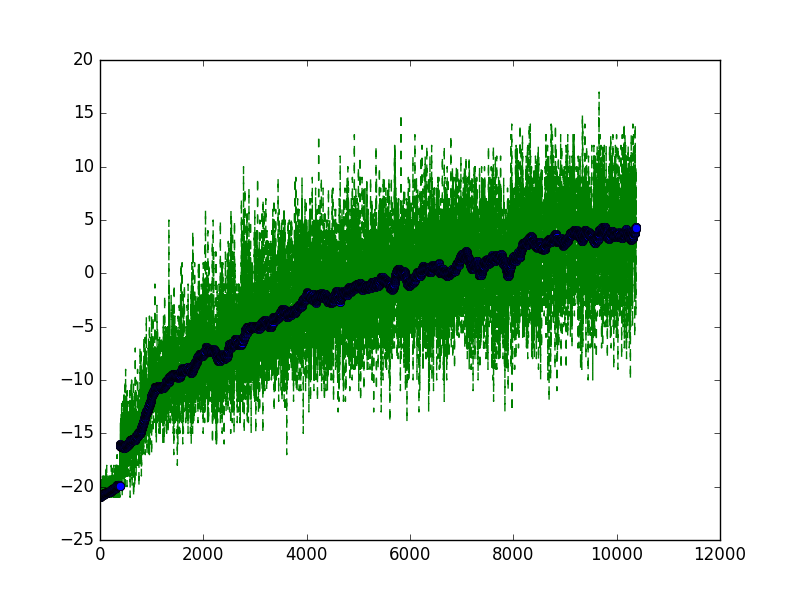
\includegraphics[width=0.49\textwidth]{./fig/pg_pong_rewardsplot.png} 
\caption{The plot of reward for pong game. The x-axis is the number
of episodes it has been trained. The y-axis is the cumulative reward in 
per episode. The higher the better. }
\label{fig:pg_pong}
\end{figure}




\subsubsection{Asynchronous advantage actor-critic}
The experimental results are illustrated in the Fig~\ref{fig:A3C_baselines}. Please also
see the video animation by clicking the captions under each figures. 
% The results are acquired by a pre-trained model and then follow the A3C models,

\begin{figure}[h!]
\centering
\begin{tabular}{c}
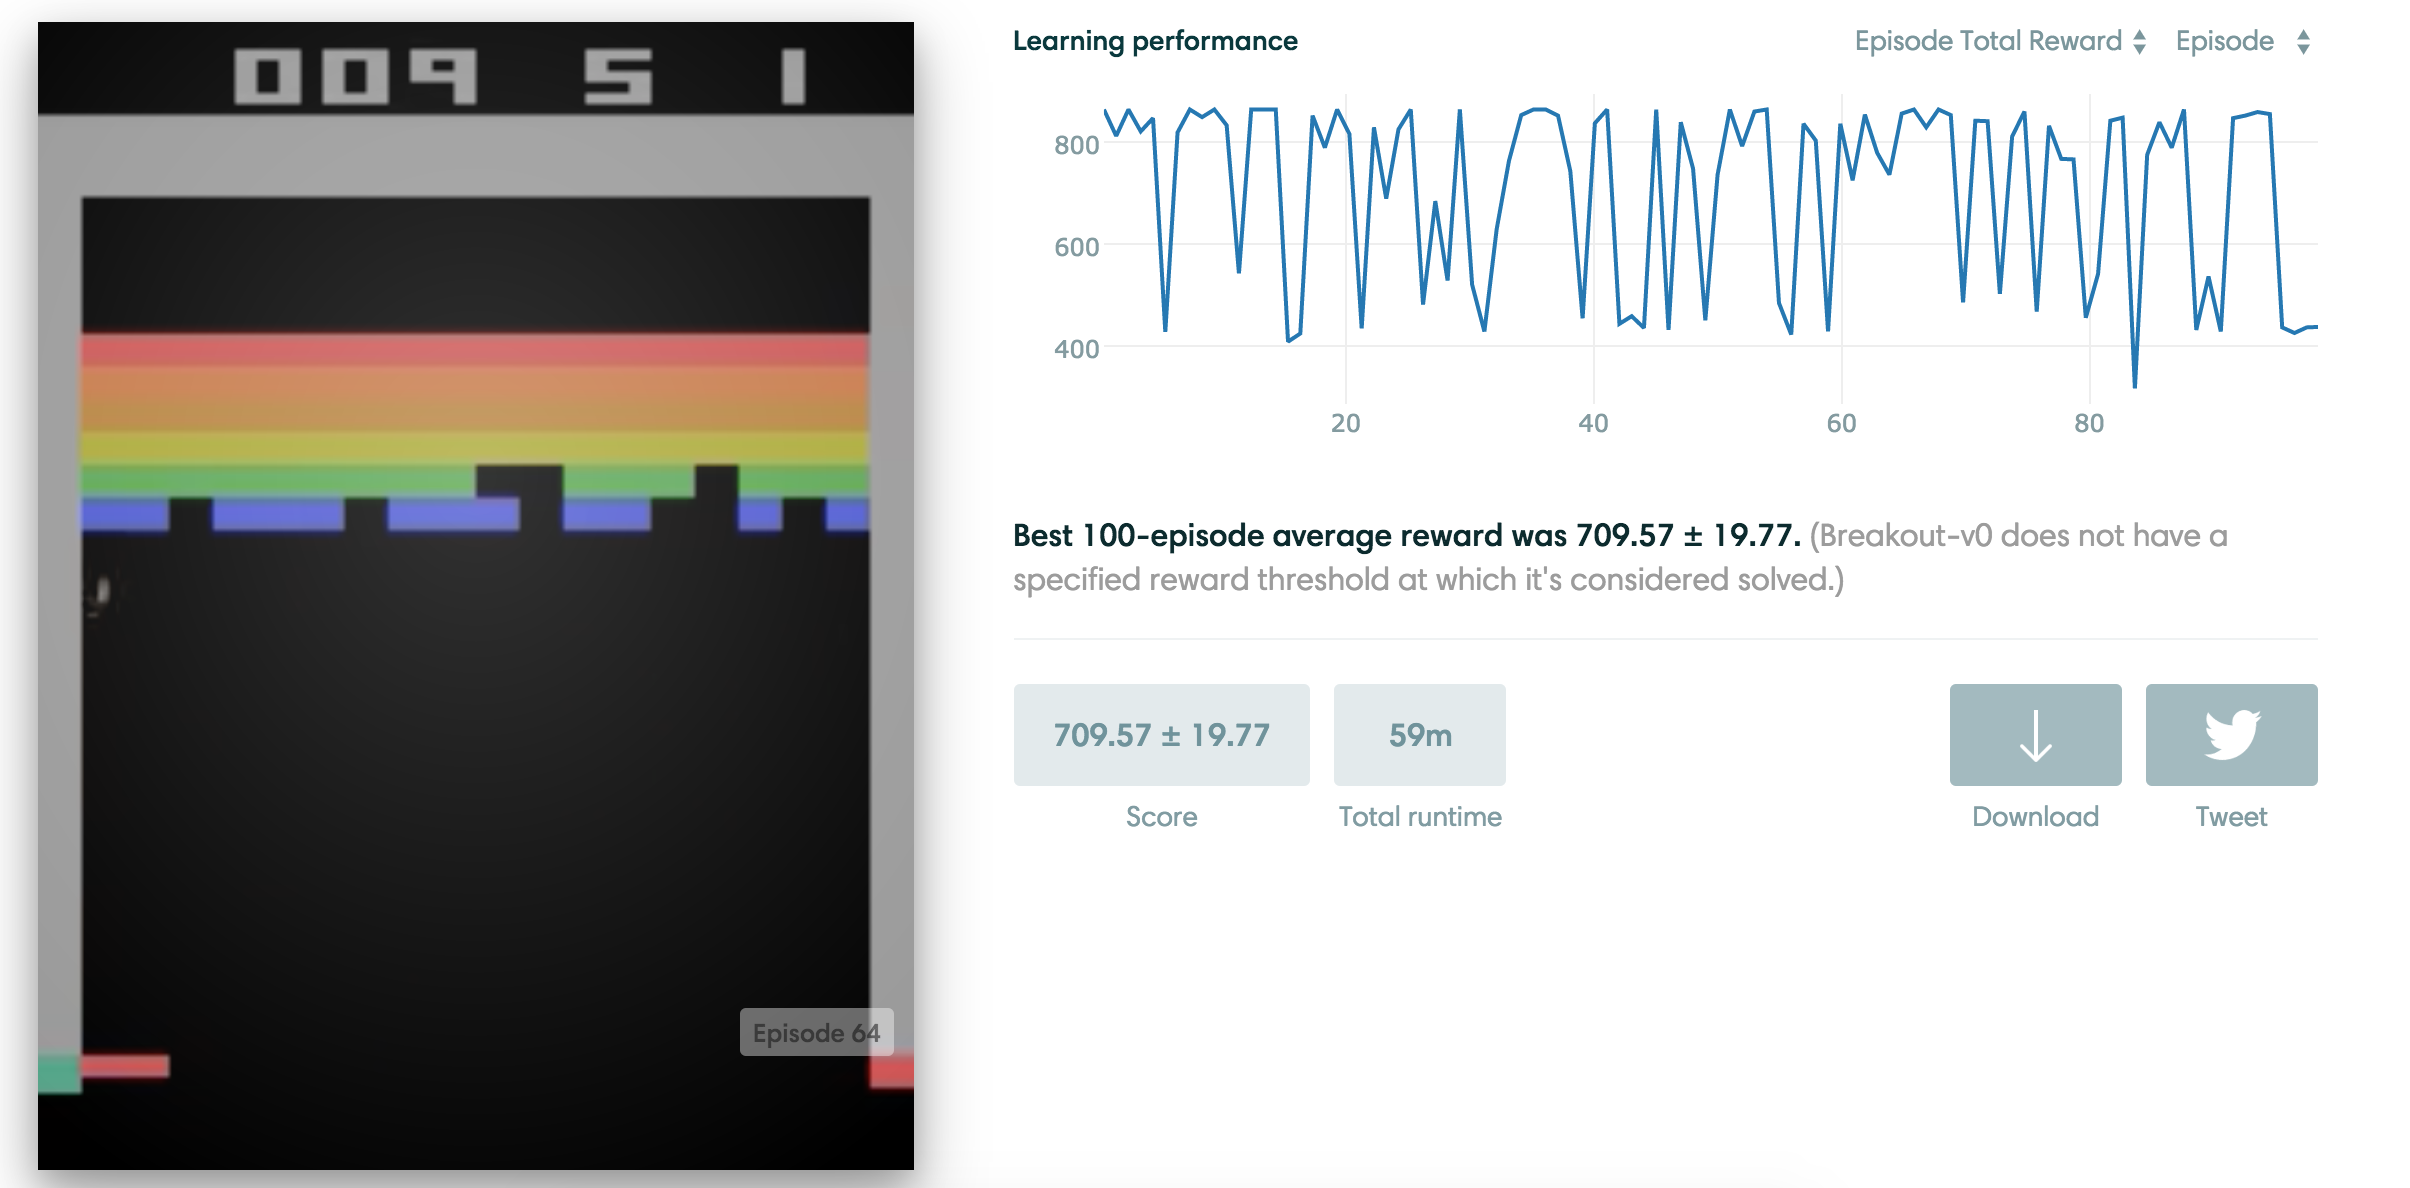
\includegraphics[width=0.49\textwidth]{./fig/A3C_Breakout-v0.png} \\
(a) \href{https://gym.openai.com/evaluations/eval_i9E40nAQuOTiSa0bxYBA#reproducibility}{Breakout-v0} \\
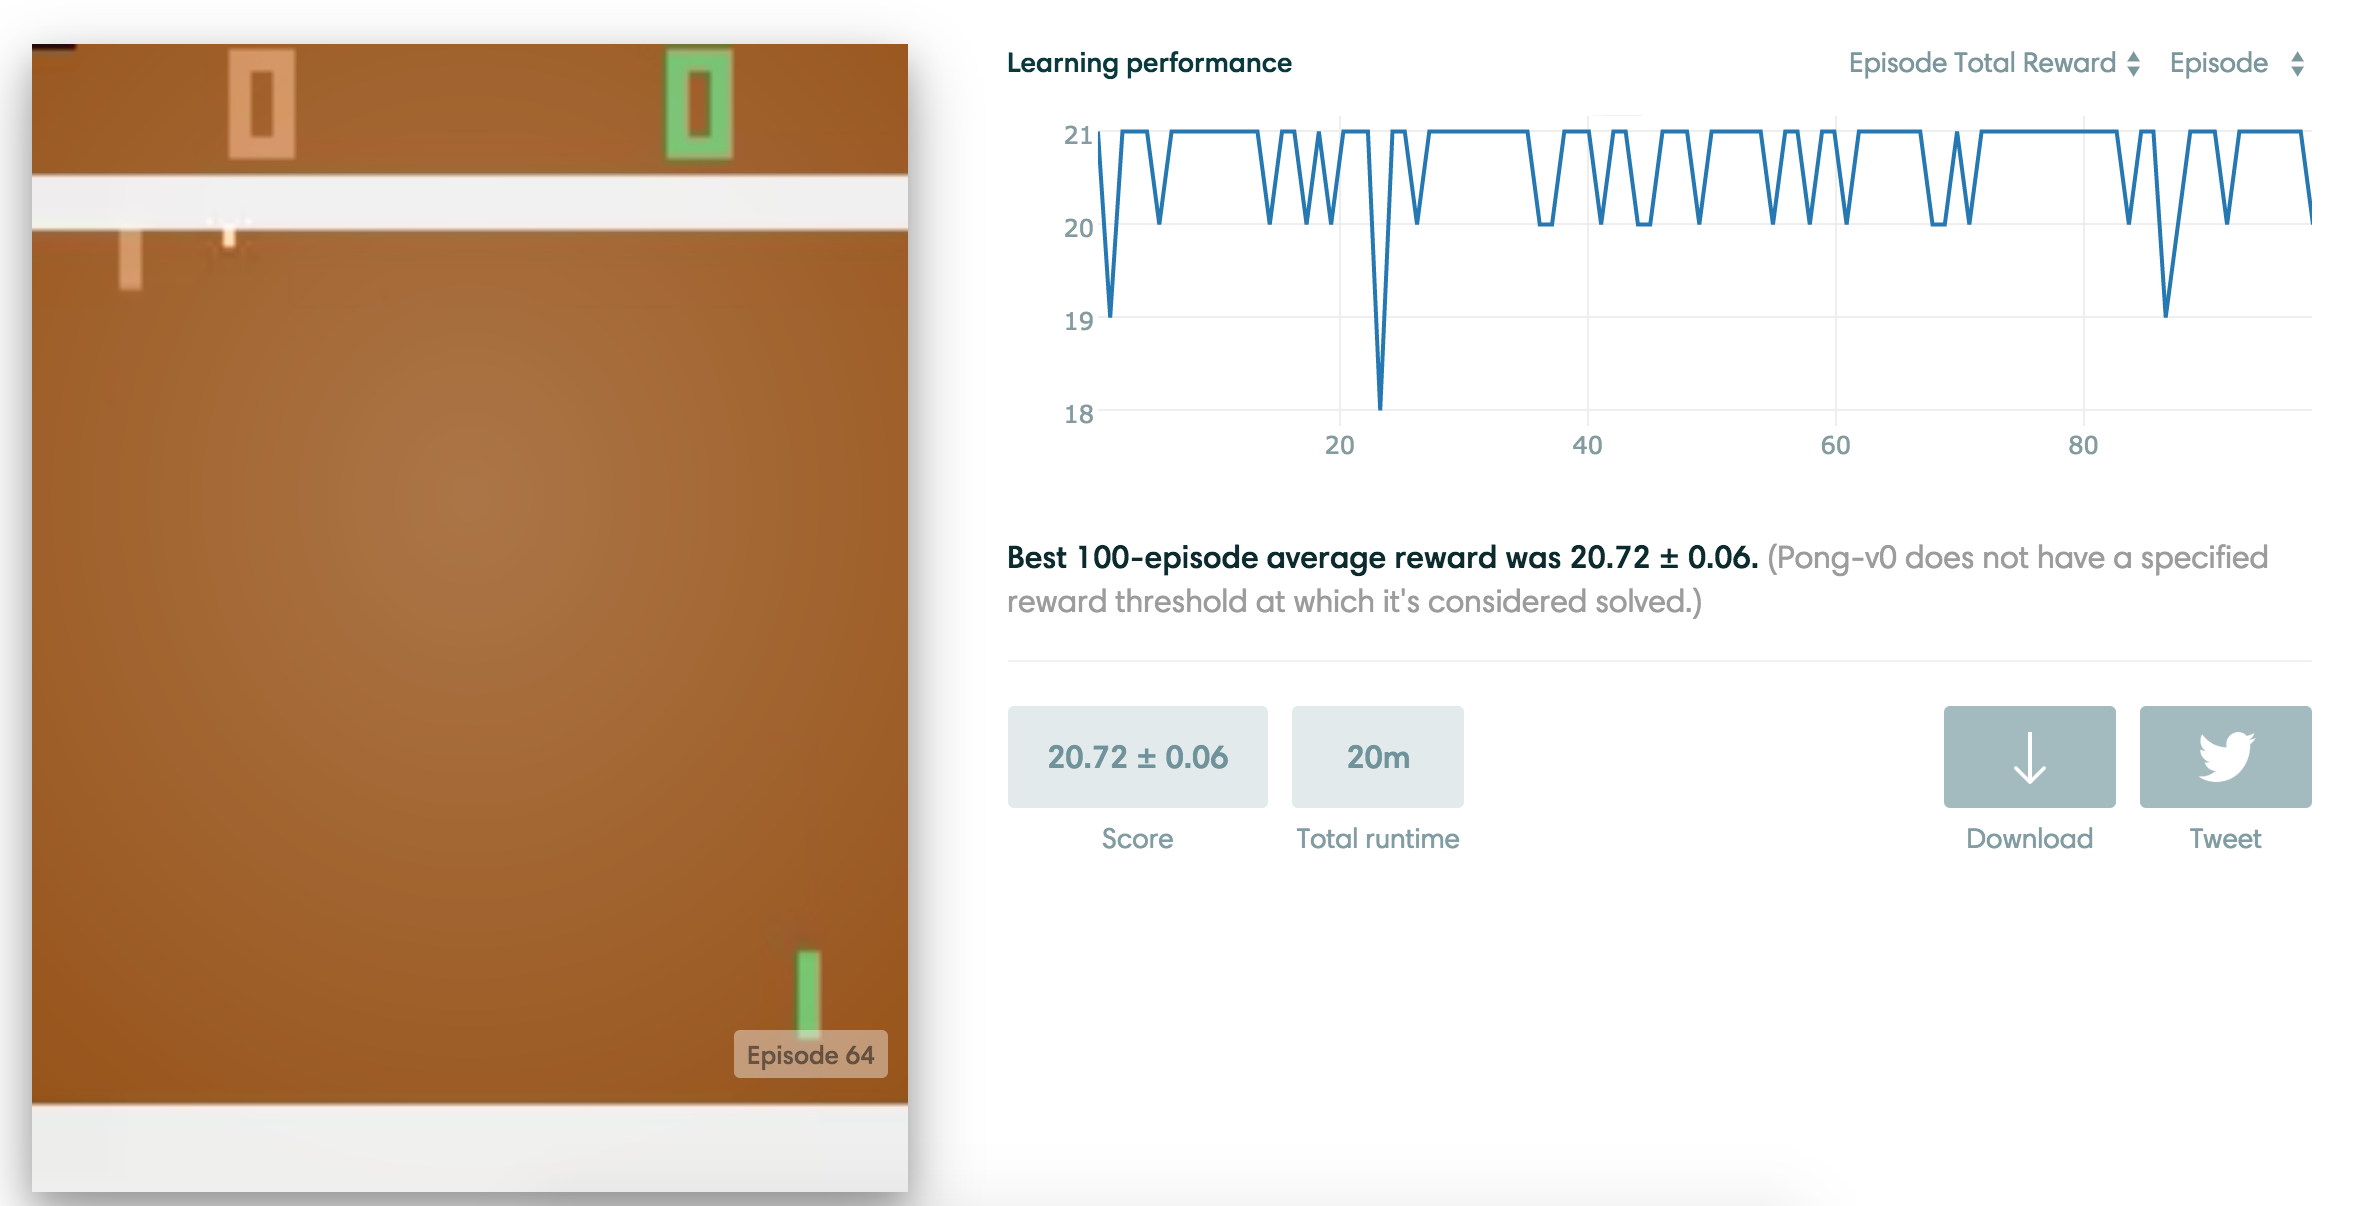
\includegraphics[width=0.49\textwidth]{./fig/A3C_Pong-v0.png} \\
(b) \href{https://gym.openai.com/evaluations/eval_mvXuxP13SSacO01UIhsg#reproducibility}{Pong-v0} \\
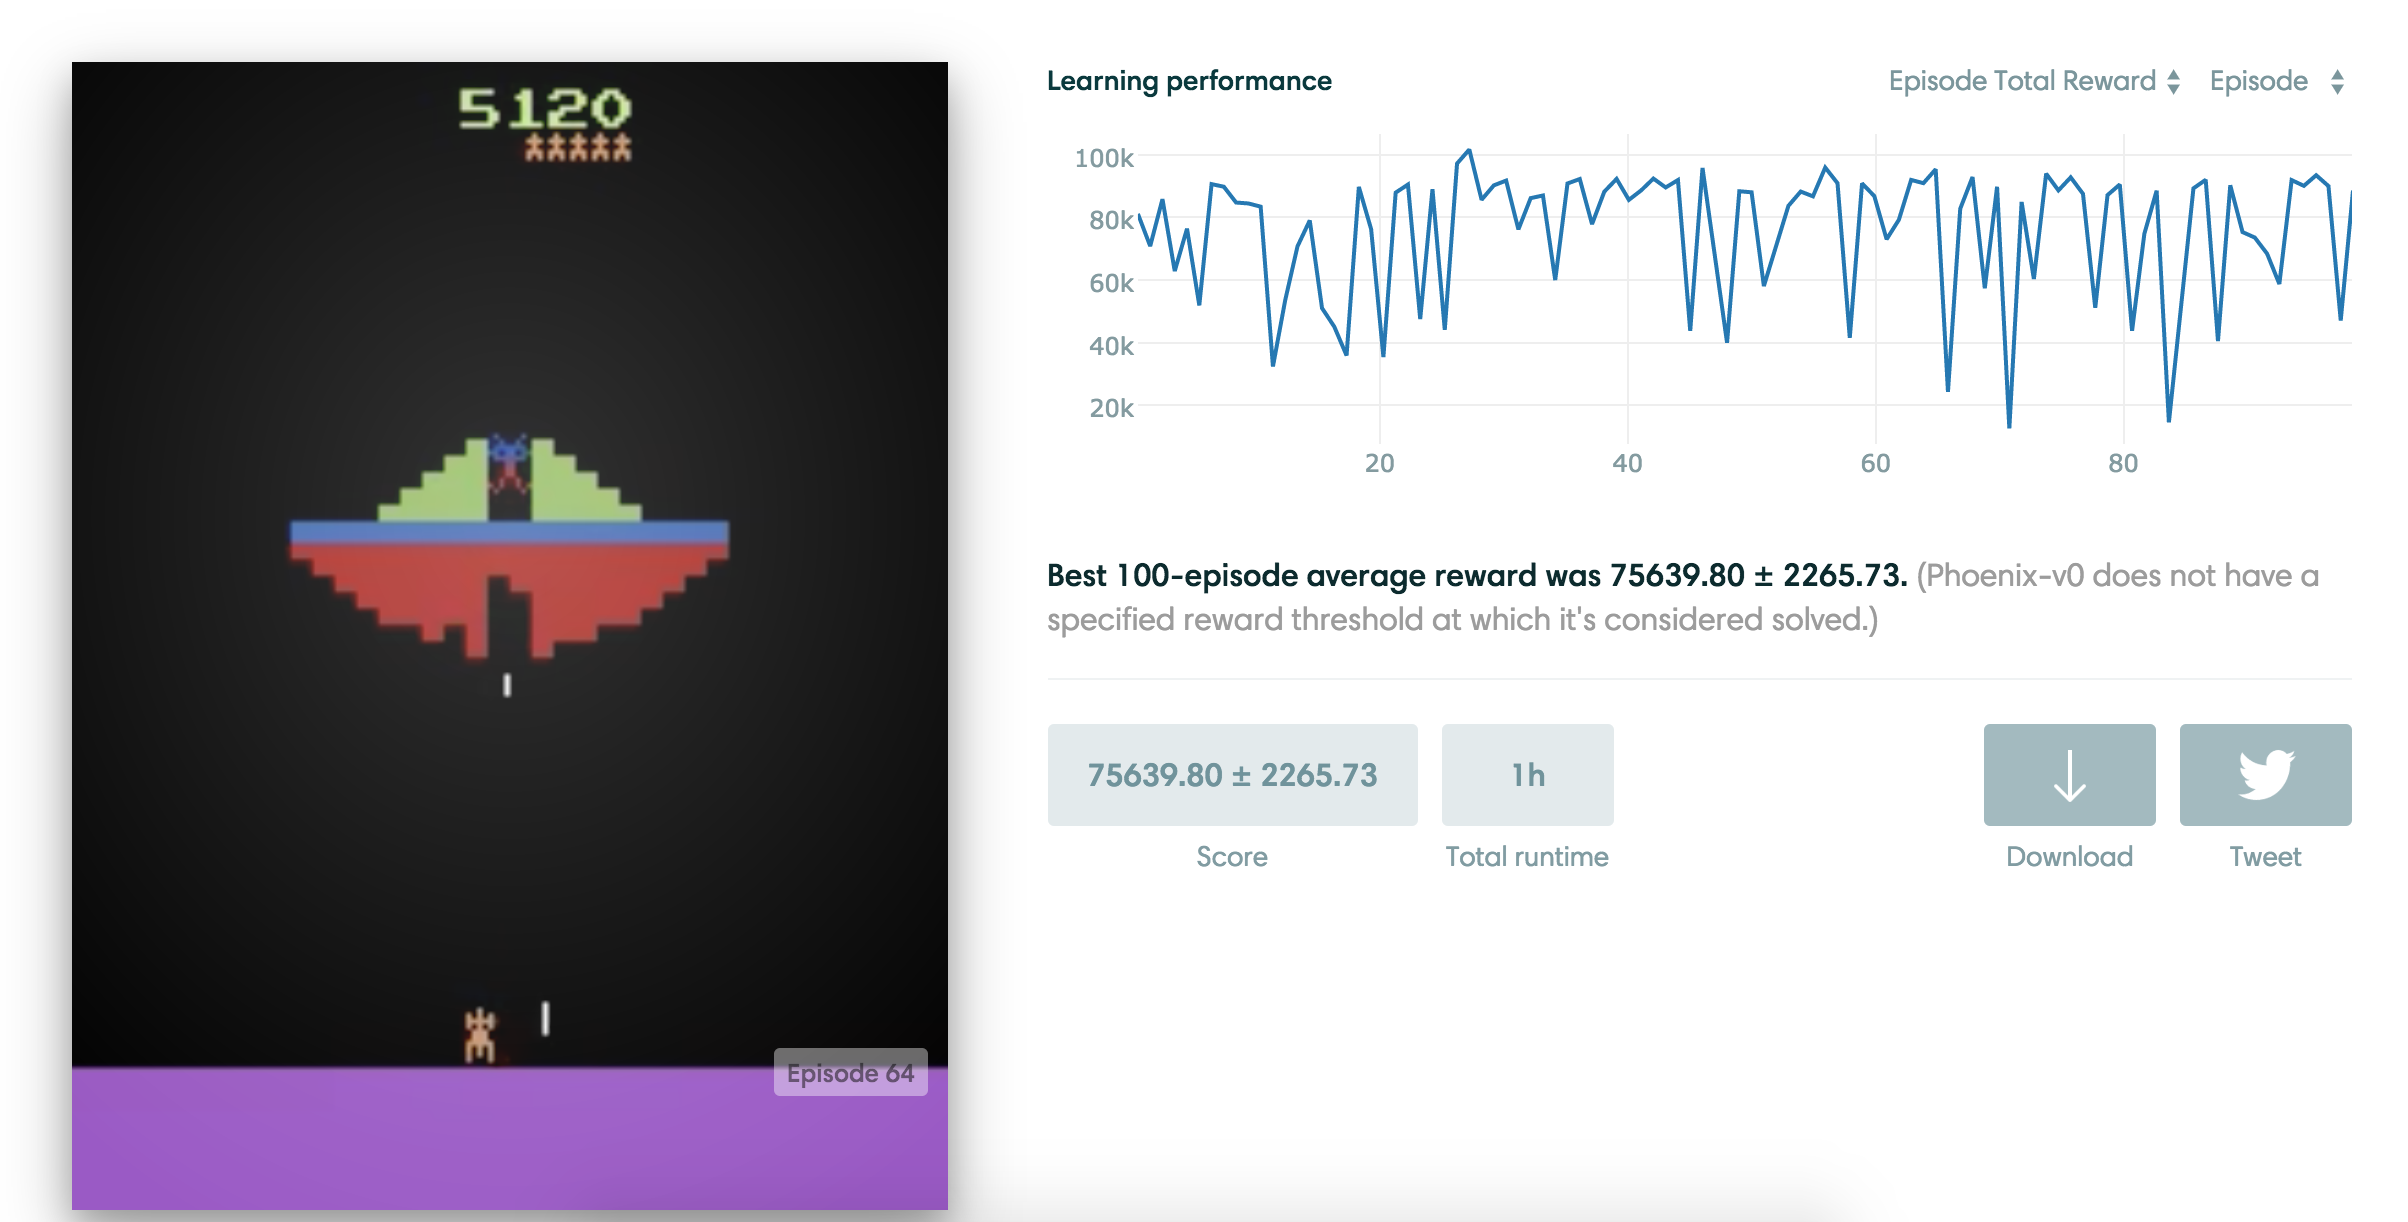
\includegraphics[width=0.49\textwidth]{./fig/A3C_Phoenix-v0.png} \\
(c) \href{https://gym.openai.com/evaluations/eval_Gva8XrEvTQi63KOd5Gyq1Q#reproducibility}{Phoenix-v0} \\
\end{tabular}
\caption{The results of 100 epsiodes on three environments by applying A3C algorithms. By clicking the name of each environment 
beneath the figures, you will see the video for each game played by trained agent.}
\label{fig:A3C_baselines}
\end{figure}



